\section{Userspace}
\subsection{sys/class/gpio}
\begin{frame}{\cod{sys/class/gpio}}
 \begin{itemize}
  \item \cod{kernel/Documentation/gpio.txt}
  \item Gute Pins:
   \begin{itemize}
    \item 35: PWR\_LED
    \item 47: ACT\_LED
   \end{itemize}
 \end{itemize}
\end{frame}

\subsection{mmap}
\begin{frame}{\cod{mmap}}{Direkter Zugriff auf die Hardware}
 \begin{itemize}
  \item Beschreibung
   \begin{itemize}
    \item BCM2835 ARM Peripherals (BCM2835-ARM-Peripherals.pdf) Abschnitt 6
   \end{itemize}
  \item Wo im Speicher
   \begin{itemize}
    \item \cod{/proc/iomem}
   \end{itemize}
 \item Der wichtige Aufruf
  \begin{itemize}
   \item \cod{mmap}
  \end{itemize}
 \end{itemize}
\end{frame}

\begin{frame}[fragile]{mmap}
\begin{center}
 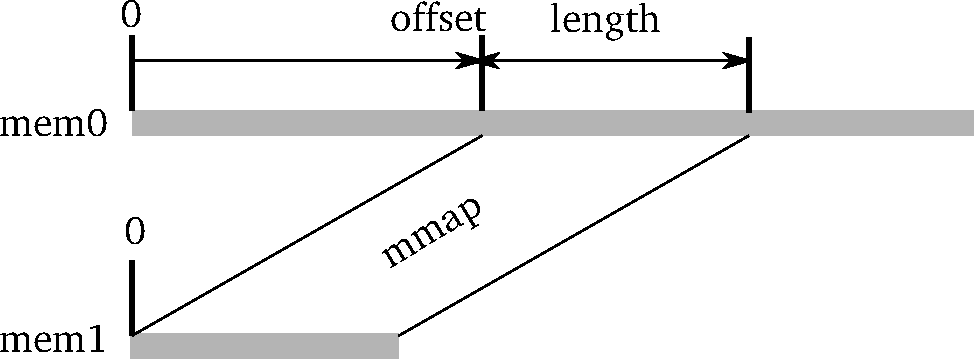
\includegraphics[width=8cm]{mmap.pdf}
\end{center}
\begin{lstlisting}[language=C]
 mem=(unsigned char*)mmap(0, /* addr hint */
     length,
     PROT_READ|PROT_WRITE,
     MAP_SHARED, 
     memId,
     offset);
\end{lstlisting}
\end{frame}

\subsection{Aufgaben}
\begin{frame}{Aufgaben}
 \begin{itemize}
  \item \cod{gpio.sh}:  \cod{sys/class/gpio}
  \item \cod{blink.sh}: \cod{mmap}/\cod{direct-memory.cc}
  \item \cod{blink} als \cpp Programm mit Module \cod{mmap.h|cc}
 \end{itemize}
\end{frame}
